

\section{Introduction}

The measurement of frequency response functions (FRFs) of dynamic systems is an important topic in the measurement society.  FRF measurement techniques are discussed, for instance, in 
\cite{Schoukens1998ImprFRFmeas,schoukens2006leakagereduction,guillaume1996,broersen1995transferfunction,pintelon2010lpm1,Antoni20071723,FDidentEd2Pintelon}, and applied to real practical devices and systems \cite{Lim2010,Robinson1990,Behjat2010}, among others. Besides, FRFs have been shown to provide a quick insight into the dynamic properties of linear-time-invariant (LTI) systems. This capability is very useful for model validation and/or selection \cite{FDidentEd2Pintelon}.

This paper uses nonparametric models in conjunction with the local polynomial method (LPM) \cite{pintelon2010lpm1} to estimate the complex frequency response function (FRF) in a linear-least-squares (LS) sense. The advantage of using the nonparametric models is basically the non-involvement of the user in choosing a model order, i.e. no user interaction. Among the current nonparametric methods, the LPM method is chosen due to its superiority over the classical nonparametric methods (windowing) in suppressing leakage errors \cite{bendatPiersol1993,Oppenheim1983}. Consequently, the LPM estimate of the FRF is not hampered by leakage errors \cite{pintelon2010lpm1,schoukens2010nonparametric}. Note that a more general discussion on the LPM, applied to noisy, real-valued data is found in \cite{fanGijbels1996LPM} with a specific focus on parametric tuning.

The main contribution of the paper is to come up with an improved FRF by developing a method for smoothing the FRF estimated via the LPM. This is done by truncating the associated impulse response, as in \cite{Schoukens1998ImprFRFmeas}, but with the following additional extension: the determination of the optimal truncation time, without any user interaction, in conjunction with the use of the LPM for leakage reduction. The cutoff index (truncation point) is determined by a statistically sound method. It is then shown that a smooth LPM estimate of the FRF lowers the variance, thus improving the assessment level of the dynamic properties of a given LTI system. 

Based on \cite{schoukens2010nonparametric}, the nonparametric method developed in this work is formulated in an output-error (OE) framework. A single-input-single-output (SISO) LTI system is considered. %, based on  \cite{schoukens2010nonparametric}. 
The input signal is a known random noise signal and the output signal is corrupted by measurement noise. This is depicted in Fig. 1 as a linear dynamic discrete-time SISO system, whose full mathematical model is of the form:
\begin{equation}\label{lpmtd1}
y(t)=G_0(q)u_0(t)+H_0(q)e(t)=G_0(q)u_0(t)+v(t)
\end{equation}
where $G_0(q)$ represents the dynamics of the system to be estimated, $u_0(t)$ is the input signal, $v(t)= H_0(q)e(t)$ is the noise source at the output, $H_0(q)$ is the noise dynamics, $e(t)$ is white noise, and $q^{-m}$ is the backwards shift operator ($q^{-m}x(t)$ = $x(t-m)$  with $m$ a positive integer). %\JL{$G_0(q)$ represents the dynamics of the system to be estimated.}

\begin{figure}[tbh] %top bottom here
\centering
%\tikzstyle{block}     = [draw,rectangle,minimum height=2em,minimum width=1.5em,inner sep=2mm]
\tikzstyle{sum}       = [draw,circle,inner sep=0mm,minimum size=2mm]
\tikzstyle{input} = []
\tikzstyle{output} = []
\tikzstyle{pinstyle} = [pin edge={<-,black},color=black]

\begin{tikzpicture}[auto, node distance=2cm,>=latex]

    \node [near start] (input) {$\true{u}(t)$};
    \node [block, right of=input] (system) {$\true{G}(q^{-1})$};
    \node [sum, right of=system,
           node distance=2.2cm] (sum) {\footnotesize$+$};
    \node [right of=sum, node distance=1.3cm] (output) {$y(t)$};

    \node [above of=sum, node distance=1.3cm] (noise) {$v(t)$};

    \draw [->] (input)  --   (system);
    \draw [->] (system) -- node[name=y0] {$\true{y}(t)$} (sum);
    \draw [->] (sum)    --    (output);

    \draw [->] (noise) -- (sum);

\end{tikzpicture}

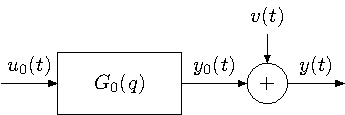
\includegraphics{tikz0.pdf}
\caption{SISO LTI discrete-time system in an output error setup.}
\label{lpmtdrep}
\end{figure}

Numerous parametric identification techniques are devoted to the development of parametric plants $G(q,\theta)$ and parametric noise models  $H(q,\theta)$, where  $\theta$ is the model parameters vector  \cite{Ljung1999,Soderstrom1989}. 

In this paper, however, a nonparametric technique is developed, %the identification problem is 
formulated in the frequency domain, consistent with \cite{FDidentEd2Pintelon,Mahata2006}. The following  choices are made:

\begin{itemize}

\item

The work in this paper is for discrete-time systems. Denote the $k^{th}$ discretized frequency as $\Omega_k$ = $e^{-j2{\pi}kf_s/N}$, with $f_s$ the sample frequency and $N$ the total number of sample points.
\item

Describe the parametric plant model  $G(q,\theta)$ by the nonparametric FRF counterpart  $G(\Omega_k)$  at the $k^{th}$ frequency. 
\item

Describe  the parametric noise model $H(q,\theta)$ (associated with the output noise source $v(t)$) by a nonparametric noise variance contribution $\sigma^2_v(\Omega_k)$ at the $k^{th}$ frequency.

\end{itemize}

The rest of the paper is structured as follows. Section \ref{se:theoryLPMandWindowing} covers the theory on the LPM and windowing for an OE setup. 
Section \ref{se:smoothingFRFestimate} discusses the novel smoothing method. 

Ultimately, in Section \ref{se:simResults}, simulation results of the following FRF estimates and their corresponding variances are compared: (i) the smooth LPM estimate $\hat{G}_\text{sm-poly}(\Omega_k)$, (ii) the LPM estimate $\hat{G}_\text{poly}(\Omega_k)$. 

These FRF estimates are also compared with the true LTI system ${G}_0(\Omega_k)$. Discussion of the simulation results is then followed by a conclusion in Section \ref{se:conclusion}.

